% ============================================================
%  Chapter 3: Bracketing
%  Algorithms for Optimization, 2nd ed., 2026
%  Kochenderfer & Wheeler
%  Beamer slides (16:9, Madrid/seahorse)
%  Reader-friendly edition -- complete explanatory prose
% ============================================================
\documentclass[aspectratio=169,10pt]{beamer}

\usetheme{Madrid}
\usecolortheme{seahorse}

\usepackage{amsmath,amssymb,amsthm}
\usepackage{mathtools}
\usepackage{listings}
\usepackage{xcolor}
\usepackage{graphicx}
\usepackage{booktabs}
\usepackage{tikz}
\usepackage{hyperref}

\graphicspath{{figures/}}

% ------------------------------------------------------------------
% Python listing style
% ------------------------------------------------------------------
\lstdefinestyle{pycode}{
  language=Python,
  basicstyle=\ttfamily\scriptsize,
  numbers=left,
  numberstyle=\tiny\color{gray},
  stepnumber=1,
  numbersep=4pt,
  frame=single,
  backgroundcolor=\color{gray!7},
  keywordstyle=\color{blue!70!black}\bfseries,
  commentstyle=\color{green!50!black}\itshape,
  stringstyle=\color{red!60!black},
  showstringspaces=false,
  breaklines=true,
  tabsize=4,
  captionpos=b,
  aboveskip=2pt,
  belowskip=2pt
}

\setbeamertemplate{footline}[frame number]
\setbeamertemplate{navigation symbols}{}

% ------------------------------------------------------------------
% Title
% ------------------------------------------------------------------
\title[Chapter 3: Bracketing]{\textbf{Chapter 3: Bracketing}}
\subtitle{Algorithms for Optimization, 2nd Edition (2026)}
\author{Kochenderfer \& Wheeler}
\institute{Lecture Slides}
\date{}

% ==================================================================
\begin{document}
% ==================================================================

\begin{frame}
  \titlepage
\end{frame}

% ------------------------------------------------------------------
\begin{frame}{Outline}
  \tableofcontents
\end{frame}

% ==================================================================
\section{Introduction \& Motivation}
% ==================================================================

\begin{frame}[allowframebreaks]{What Is Bracketing?}

  Optimization often begins not with a precise answer, but with a \emph{region}
  in which we believe the answer lives.  Bracketing is the systematic process of
  constructing and shrinking that region.

  \begin{block}{Definition: Bracketing}
    \textbf{Bracketing} is the process of identifying an interval $[a, c]$ ---
    read ``the interval from $a$ to $c$'' --- within which a local minimum is
    guaranteed to lie, and then progressively narrowing that interval until the
    minimum is located to the desired precision.  Here $a$ (the left endpoint)
    and $c$ (the right endpoint) are real numbers with $a < c$.
  \end{block}

  Bracketing applies to \textbf{univariate} functions --- functions that take a
  single real-valued input $x$ and return a single real-valued output $f(x)$.
  The central idea is simple: if we know the minimum is somewhere inside $[a,c]$,
  we can evaluate $f$ at one or two interior points, learn something about the
  shape of $f$, and discard part of the interval where the minimum cannot be.
  Repeating this procedure drives the interval length toward zero.

  Derivative information (the slope $f'(x)$ of the function) can accelerate
  the search when available, but several of the methods in this chapter work
  with \textbf{function values alone} --- they treat $f$ as a ``black box''
  that can only be queried at chosen points.

  The methods studied in this chapter form the foundation for
  \textbf{line search} in multi-variable optimization (Chapter 4 onward):
  minimizing along a direction in higher-dimensional space reduces to a
  one-dimensional bracketing problem.

  \begin{alertblock}{Key Insight}
    We do not need to evaluate $f$ everywhere.  A handful of cleverly placed
    evaluations, combined with the right structural assumption about $f$
    (such as unimodality, defined next), is enough to converge on the minimum.
  \end{alertblock}

\end{frame}

% ==================================================================
\section{Unimodality}
% ==================================================================

\begin{frame}[allowframebreaks]{3.1\ \ Unimodality}

  Before we can safely discard part of a bracketing interval, we need to know
  that discarding it will not accidentally throw away the true minimum.
  \emph{Unimodality} is the key assumption that makes this safe.

  \begin{block}{Definition: Unimodal Function}
    A function $f$ is \textbf{unimodal} (``one-humped'', from the Latin
    \textit{unus} = one, \textit{modus} = mode/peak) if there exists a unique
    minimizer $x^{*}$ (read ``$x$ star'', meaning the optimal point) such that:
    \[
      f \text{ is strictly \emph{decreasing} for all } x \le x^{*}
      \qquad\text{and}\qquad
      f \text{ is strictly \emph{increasing} for all } x \ge x^{*}.
    \]
    In other words, the function has exactly one ``valley'' and no other local
    minima.  Moving left from $x^{*}$ always increases $f$; moving right from
    $x^{*}$ also always increases $f$.
  \end{block}

  A helpful mental image: think of a bowl.  No matter where you start inside
  the bowl, the floor is at one unique lowest point.  A function like
  $f(x) = (x-2)^2$ is unimodal with minimum at $x^{*} = 2$.

  \begin{block}{Definition: Multimodal Function}
    A \textbf{multimodal} function has multiple local minima (multiple
    ``valleys'').  For example, $f(x) = \sin(x)$ is multimodal: it dips down
    to $-1$ repeatedly.  Most bracketing methods in this chapter \emph{cannot}
    be directly applied to multimodal functions without additional global
    search strategy.
  \end{block}

  Unimodality gives us a powerful tool: if we find three points
  $a < b < c$ (read ``$a$ strictly less than $b$ strictly less than $c$'')
  where the \emph{middle} value is lower than both ends, the minimum
  \emph{must} lie between the outer points.

  \begin{block}{Definition: Bracket for a Unimodal Function}
    Given a unimodal function $f$, an interval $[a, c]$ \textbf{brackets} the
    global minimum if there exists a point $b$ with $a < b < c$ satisfying
    \[
      f(a) > f(b) \quad \text{and} \quad f(b) < f(c).
    \]
    Here $f(a)$ means ``the value of $f$ evaluated at the point $a$'', and the
    two inequalities together say that $b$ sits lower than both endpoints.
    We call the triple $(a, b, c)$ a \textbf{bracketing triple}.
  \end{block}

  Why does this work?  Because $f$ is unimodal, the shape of the function
  everywhere to the left of $b$ is monotonically decreasing (values going
  down as we approach $b$) and everything to the right of $b$ is
  monotonically increasing (values going up as we move away from $b$).
  The minimum cannot be outside $[a, c]$ without violating this monotone
  structure.

  \begin{alertblock}{Key Insight}
    The unimodality assumption is what makes bracketing methods \emph{safe}:
    once we have a valid triple $(a, b, c)$ with $f(a) > f(b) < f(c)$,
    every subsequent evaluation can only tighten the bracket, never lose
    the minimum.
  \end{alertblock}

\end{frame}

\begin{frame}[allowframebreaks]{Visualizing a Bracket}

  The figure below shows a unimodal function with a valid bracketing triple.
  The point $b$ in the middle has a lower function value than both $a$ on
  the left and $c$ on the right.  This configuration \emph{proves} the
  minimum lies somewhere in $[a, c]$.

  \begin{center}
    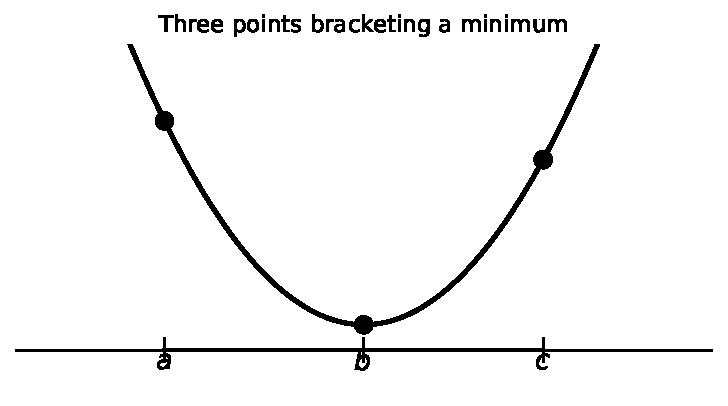
\includegraphics[width=0.75\textwidth]{fig_unimodal_bracket}
  \end{center}

  Reading the figure: the horizontal axis is the input $x$, the vertical
  axis is the output $f(x)$.  The three labeled points $a$, $b$, $c$ are
  marked on the $x$-axis, and the dots above them show the corresponding
  function values.  Because the dot above $b$ is the lowest of the three,
  the triple is a valid bracket.  The shaded region $[a, c]$ is where
  we continue to look for the minimum.

\end{frame}

% ==================================================================
\section{Finding an Initial Bracket}
% ==================================================================

\begin{frame}[allowframebreaks]{3.2\ \ Finding an Initial Bracket}

  Before applying a refinement method such as Fibonacci or Golden Section
  search, we first need a valid bracketing triple $(a, b, c)$.  This section
  describes a simple but robust algorithm that \emph{finds} an initial bracket
  by probing the function.

  The strategy is intuitive: start at some point $x_0$ (x sub zero, our initial
  guess) and take a small step in the positive direction.  If the function goes
  \emph{up}, the minimum is to the left, so we reverse direction.  Then we
  march forward, doubling our step size at each iteration, until we find a
  point where the function starts going back up.  At that moment we have a
  bracket: the point before the upturn, the current point, and the previous
  point form a valid triple.

  \begin{block}{Algorithm 3.1 --- \texttt{bracket\_minimum}$(f,\; x_0;\; s,\; k)$}
    \textbf{Inputs:}
    \begin{itemize}
      \item $f$ --- the function to minimize (a callable that takes a real number)
      \item $x_0$ (x sub zero) --- starting point, default $0$
      \item $s$ --- initial step size, default $10^{-2}$ (a small positive number)
      \item $k$ (kappa) --- step expansion factor, default $2$
    \end{itemize}
    \textbf{Output:} an interval $[a, b]$ that brackets a local minimum.\\[4pt]
    \textbf{Procedure:}
    \begin{enumerate}
      \item Set $a \leftarrow x_0$,\; $y_a \leftarrow f(a)$;\quad
            set $b \leftarrow a + s$,\; $y_b \leftarrow f(b)$.
            (The arrow $\leftarrow$ means ``assign the value on the right to the variable on the left''.)
      \item If $y_b > y_a$ (the step went uphill): swap $a$ and $b$, swap
            $y_a$ and $y_b$, and negate $s$ (reverse direction).
      \item \textbf{Repeat} the following until a bracket is found:
        \begin{itemize}
          \item Set $c \leftarrow b + s$,\; $y_c \leftarrow f(c)$.
          \item If $y_c > y_b$ (another uphill step): the minimum is between
                the previous two points, so \textbf{return} the sorted interval.
          \item Otherwise, advance: set $a \leftarrow b$, $y_a \leftarrow y_b$,
                $b \leftarrow c$, $y_b \leftarrow y_c$.
          \item Expand: set $s \leftarrow k \cdot s$ (multiply the step by $k$,
                i.e., double it when $k=2$).
        \end{itemize}
    \end{enumerate}
  \end{block}

  \begin{block}{Notation}
    $x_0$ (x sub zero): the starting point, a single real number.\\
    $s$: the current step size, in the same units as $x$.\\
    $k$ (kappa, the Greek letter for ``k''): the expansion multiplier --- each
    step is $k$ times longer than the previous one, so the search grows
    exponentially.\\
    $y_a, y_b, y_c$: the function values $f(a)$, $f(b)$, $f(c)$ stored for
    reuse (to avoid re-evaluating $f$, which may be expensive).
  \end{block}

  \begin{alertblock}{How to Read This Algorithm}
    Think of a hiker on a hillside who cannot see the whole landscape.  She
    takes a step forward.  If it went uphill, she turns around.  She then
    starts walking with increasingly long strides until she takes a step and
    finds herself going uphill again --- at that point she knows the valley is
    somewhere behind her last two positions.\\[4pt]
    The exponential expansion ($k=2$) is crucial: it ensures the algorithm
    terminates in $O(\log(\text{distance to minimum}))$ steps rather than
    crawling at constant step size.
  \end{alertblock}

  \textbf{Important Caveat:} Functions that have \emph{no} local minimum on
  $(-\infty, +\infty)$ --- for example $f(x) = e^x$, which decreases forever
  to the left --- will cause this algorithm to run indefinitely.  Always
  ensure the function has a minimum before calling it.

\end{frame}

\begin{frame}[fragile]{Python: \texttt{bracket\_minimum}}
\begin{lstlisting}[style=pycode, caption={Python equivalent of Algorithm 3.1}]
import numpy as np

def bracket_minimum(f, x=0.0, s=1e-2, k=2.0):
    """Find an interval [a, b] bracketing a local minimum of f.

    Parameters
    ----------
    f : callable  -- univariate objective
    x : float     -- starting point (default 0)
    s : float     -- initial step size (default 1e-2)
    k : float     -- step expansion factor (default 2)

    Returns
    -------
    (a, b) : tuple of floats
    """
    a, ya = x, f(x)
    b, yb = a + s, f(a + s)

    if yb > ya:                     # wrong direction -- reverse
        a, b = b, a
        ya, yb = yb, ya
        s = -s

    while True:
        c, yc = b + s, f(b + s)
        if yc > yb:                 # found a bracket
            return (a, c) if a < c else (c, a)
        a, ya, b, yb = b, yb, c, yc
        s *= k                      # expand step
\end{lstlisting}
\end{frame}

\begin{frame}[allowframebreaks]{Bracket Minimum: Example Iterations}

  The figure below shows four successive stages of the
  \texttt{bracket\_minimum} algorithm on a sample function.

  \begin{center}
    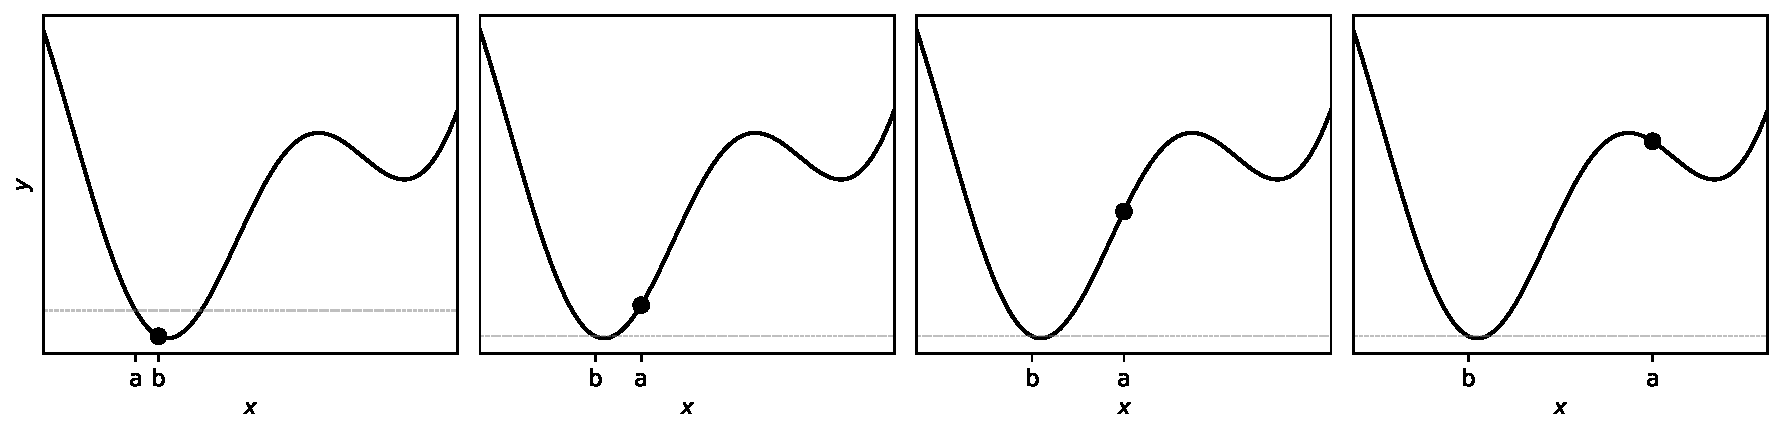
\includegraphics[width=0.90\textwidth]{fig_bracket_minimum}
  \end{center}

  Reading the panels from left to right:
  \begin{itemize}
    \item \textbf{Panel 1 (leftmost):} The algorithm takes an initial step to
          the right and finds the function value went \emph{up}.  It therefore
          reverses direction ($s \leftarrow -s$) and begins marching left.
    \item \textbf{Panels 2--3:} Each subsequent step covers twice the distance
          of the previous one ($k=2$, so the step doubles each iteration).
          The function values are still decreasing, so no bracket has been
          found yet.
    \item \textbf{Panel 4 (rightmost):} The algorithm takes a step and the
          function value increases.  This confirms a bracket: the minimum lies
          between the second-to-last and last points, and the step before that
          confirms the left side.  The algorithm returns this interval.
  \end{itemize}

  The step size doubling is what makes this algorithm efficient: even if
  the minimum is far from the starting point, the algorithm reaches it in
  a logarithmic number of steps rather than linear.

\end{frame}

% ==================================================================
\section{Fibonacci Search}
% ==================================================================

\begin{frame}[allowframebreaks]{3.3\ \ Fibonacci Search --- Key Idea}

  Once we have a valid bracketing interval $[a, b]$, we want to shrink it
  as efficiently as possible.  \textbf{Fibonacci search} answers the question:
  ``If I am allowed exactly $n$ function evaluations, where should I place
  my queries to maximally reduce the interval?''

  The answer is counterintuitive: placing both queries very close together
  near the center is nearly optimal when $n$ is large, but for a small
  fixed $n$ the optimal placement follows the Fibonacci sequence.

  \begin{block}{The Two-Query Problem}
    Suppose we have a unimodal $f$ on $[a, b]$ and we are allowed exactly
    \emph{two} function evaluations.  Where should we place them?

    If we place the queries at $\tfrac{1}{3}$ and $\tfrac{2}{3}$ of the
    interval --- that is, at points $a + \tfrac{1}{3}(b-a)$ and
    $a + \tfrac{2}{3}(b-a)$ --- then regardless of which point has the
    lower value, we can always discard exactly $\tfrac{1}{3}$ of the
    interval.  No two-query strategy can guarantee discarding more than
    $\tfrac{1}{3}$.
  \end{block}

  \begin{columns}
    \column{0.55\textwidth}
    Now consider placing the two queries infinitesimally close together
    near the center (distance $\varepsilon$ (epsilon, an infinitesimally
    small positive quantity) apart).  In this limiting case we can
    discard almost \emph{half} the interval after two evaluations.

    \medskip
    The Fibonacci strategy generalises this idea across $n$ evaluations.
    At each step, \emph{one} of the two interior points is carried over
    from the previous step (its value is already known), so we only pay
    for \emph{one new evaluation} per step.

    \column{0.42\textwidth}
    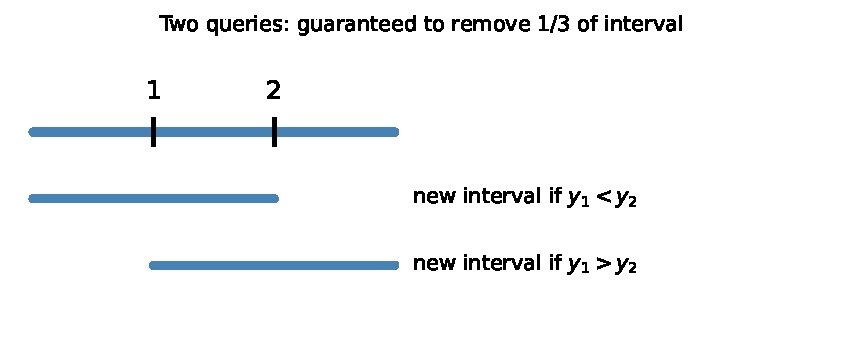
\includegraphics[width=\textwidth]{fig_fibonacci_2query}
  \end{columns}

  \begin{alertblock}{Key Insight}
    Fibonacci search is \textbf{provably optimal}: given a fixed budget of
    $n$ function evaluations on a unimodal function, no deterministic
    algorithm can guarantee a smaller final interval.  The final interval
    has length $I_1 / F_{n+1}$, where $F_{n+1}$ (F sub $n$+1) is the
    $(n+1)$-th Fibonacci number and $I_1 = b - a$ is the initial interval
    length.  Larger Fibonacci numbers mean smaller final intervals, so
    more evaluations always help --- but with diminishing returns because
    Fibonacci numbers grow exponentially.
  \end{alertblock}

\end{frame}

\begin{frame}[allowframebreaks]{Fibonacci Numbers and Interval Lengths}

  To understand Fibonacci search, we first need to understand Fibonacci
  numbers themselves and how they control interval shrinkage.

  \begin{columns}
    \column{0.55\textwidth}

    \begin{block}{Fibonacci Sequence (Eq.\ 3.1)}
      The Fibonacci sequence is defined by the recurrence relation:
      \[
        F_n =
        \begin{cases}
          1 & \text{if } n \le 2 \\
          F_{n-1} + F_{n-2} & \text{otherwise}
        \end{cases}
      \]
      where $F_n$ (F sub n) is the $n$-th term (n is an integer index
      starting at 1).  Each term is the sum of the two preceding terms.
      The first several values are: $1, 1, 2, 3, 5, 8, 13, 21, 34, \ldots$
    \end{block}

    \medskip
    After $n$ evaluations, the initial interval shrinks by the factor
    $F_{n+1}$.  For example, with $n=5$ evaluations we shrink by
    $F_6 = 8$: an interval of length $8$ becomes an interval of length $1$.

    \column{0.43\textwidth}
    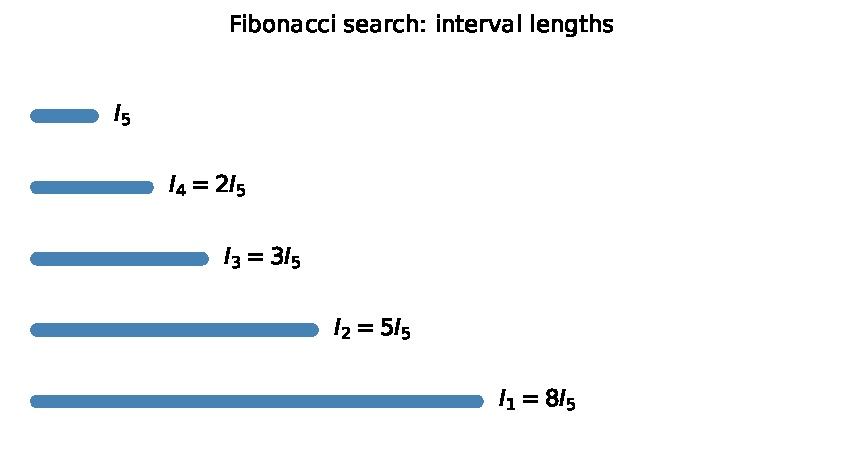
\includegraphics[width=\textwidth]{fig_fibonacci_intervals}\\[2pt]
    {\footnotesize Each row shows the interval after one more evaluation.
    The key relation is $I_1 = F_{n+1} \cdot I_n$, where $I_k$ is the
    interval length at step $k$.}
  \end{columns}

  \medskip

  \begin{block}{Binet's Formula (Eq.\ 3.2)}
    The Fibonacci numbers can be computed directly (without the recurrence)
    via Binet's formula:
    \[
      F_n = \frac{\varphi^n - (1-\varphi)^n}{\sqrt{5}},
      \qquad
      \varphi = \frac{1+\sqrt{5}}{2} \approx 1.618
    \]
    Here $\varphi$ (phi, pronounced ``fee'' or ``fye'') is the
    \textbf{golden ratio}.  The term $(1-\varphi)^n$ quickly becomes
    negligible for large $n$ (since $|1-\varphi| \approx 0.618 < 1$,
    repeated multiplication drives it toward zero), so
    $F_n \approx \varphi^n / \sqrt{5}$ for large $n$.
  \end{block}

  \begin{block}{Ratio of Successive Terms (Eq.\ 3.3)}
    The exact ratio of adjacent Fibonacci numbers used to place query
    points at step $n$ is:
    \[
      \frac{F_n}{F_{n-1}} = \varphi\,\frac{1 - s^n}{1 - s^{n-1}},
      \qquad s \approx -0.382
    \]
    where $s$ is a small correction factor (the ratio of the
    ``negligible'' term).  As $n \to \infty$ (n approaches infinity),
    this ratio converges to $\varphi$, which is the basis for Golden
    Section search in the next section.
  \end{block}

  \begin{block}{Notation Summary}
    $F_n$: the $n$-th Fibonacci number (a positive integer).\\
    $\varphi$ (phi): the golden ratio, approximately 1.618.  It satisfies
    the remarkable property $\varphi^2 = \varphi + 1$.\\
    $\sqrt{5}$: the square root of 5, approximately 2.236.\\
    $s$: a small correction factor close to $-0.382$; it is defined as
    $(1-\sqrt{5})/(1+\sqrt{5})$.
  \end{block}

\end{frame}

\begin{frame}[fragile]{Algorithm 3.2: Fibonacci Search}
\begin{lstlisting}[style=pycode, caption={Python: Fibonacci search for unimodal f on [a,b]}]
import numpy as np

def fibonacci_search(f, a, b, n, eps=0.01):
    """Fibonacci search for minimum of unimodal f on [a, b].

    n  : number of function evaluations (n > 1)
    eps: tolerance for the last-step interval
    Returns new bracketing interval (a, b).
    """
    phi = (1 + np.sqrt(5)) / 2
    s   = (1 - np.sqrt(5)) / (1 + np.sqrt(5))

    rho = 1.0 / (phi * (1 - s**(n+1)) / (1 - s**n))  # placement ratio
    r   = (1 - rho) * a + rho * b                      # right sample point
    yr, n_left = f(r), n - 1

    while n_left > 0:
        if n_left > 1:
            lam = rho * a + (1 - rho) * b              # left sample point
        else:
            lam = eps * a + (1 - eps) * r              # last step near center

        rho = 1.0 / (phi * (1 - s**(n_left+1)) / (1 - s**n_left))
        yl, n_left = f(lam), n_left - 1

        if yl < yr:
            r, b, yr = lam, r, yr        # tighten right
        else:
            a, b = b, lam                # tighten left (swap and move)

    return (a, b) if a < b else (b, a)
\end{lstlisting}
\end{frame}

\begin{frame}[allowframebreaks]{Python Code Walkthrough: Fibonacci Search}

  Let us trace through the code to understand exactly what each part does.

  \textbf{Setup (lines 1--2):}  We compute $\varphi$ (phi) as
  $(1+\sqrt{5})/2 \approx 1.618$ and the correction factor $s \approx -0.382$.
  These are the constants needed to compute the Fibonacci-optimal placement ratio.

  \textbf{Placement ratio $\rho$ (rho, pronounced ``row''):}
  The variable \texttt{rho} holds the fractional position of the first
  (right) interior query point.  A value of $\rho = 0.6$ means the point
  is placed 60\% of the way from $a$ to $b$.  The formula adjusts this ratio
  for each step so the overall strategy matches Fibonacci-optimal placement.

  \textbf{Interior points $r$ and $\lambda$ (lambda):}
  At each iteration the algorithm maintains two interior points, called
  \texttt{r} (for ``right'') and \texttt{lam} (for $\lambda$, meaning
  ``left'').  The key savings: after each step, one of these points is
  \emph{reused} in the next step.  Only \emph{one new evaluation} of $f$ is
  needed per iteration.

  \textbf{Bracket update rule:}
  \begin{itemize}
    \item If $f(\lambda) < f(r)$ (the left point is lower): the minimum is
          in $[a, r]$, so we discard everything to the right of $r$.
    \item Otherwise: the minimum is in $[\lambda, b]$, so we discard
          everything to the left of $\lambda$.
  \end{itemize}

  \textbf{Last step ($\varepsilon$ (epsilon)):}
  The final iteration uses a point very close to $r$ (at fraction $\varepsilon$
  from $a$ to $r$) to disambiguate which side of the center is lower.
  The parameter \texttt{eps} defaults to $0.01$.

\end{frame}

\begin{frame}[allowframebreaks]{Example 3.1: Fibonacci Search on $f(x) = e^{x-2} - x$}

  Let us work through a concrete numerical example to see Fibonacci search
  in action.

  \begin{block}{Problem Setup}
    We want to minimize $f(x) = e^{x-2} - x$ on the interval $[a, b] = [-2, 6]$
    using exactly $n = 5$ function evaluations.  The true minimum is at
    $x^{*} = 2$ (found by setting $f'(x) = e^{x-2} - 1 = 0$, giving
    $x = 2$).
  \end{block}

  The initial interval has length $I_1 = 6 - (-2) = 8$.  With $n=5$
  evaluations, Fibonacci search guarantees the final interval has length
  at most $I_1 / F_6 = 8/8 = 1$.

  \begin{columns}
    \column{0.52\textwidth}
    \begin{tabular}{@{}lll@{}}
      \toprule
      Evaluation & Query point $x^{(k)}$ & $f(x^{(k)})$ \\
      \midrule
      $k=1$ & $x^{(1)} = 1$ & $f(1) = e^{-1}-1 \approx -0.632$ \\
      $k=2$ & $x^{(2)} = 3$ & $f(3) = e^{1}-3 \approx -0.282$ \\
      \midrule
      \multicolumn{3}{@{}l}{$f(1) < f(3)$, so discard $[3, 6]$; new interval: $[-2, 3]$} \\
      \midrule
      $k=3$ & $x^{(3)} = 0$ & $f(0) = e^{-2}-0 \approx 0.135$ \\
      \midrule
      \multicolumn{3}{@{}l}{$f(0) > f(1)$, so discard $[-2, 0]$; new interval: $[0, 3]$} \\
      \midrule
      $k=4$ & $x^{(4)} = 2$ & $f(2) = e^{0}-2 = -1.0$ \\
      \midrule
      \multicolumn{3}{@{}l}{$f(2) < f(1)$, so discard $[0,1]$; new interval: $[1, 3]$} \\
      \midrule
      $k=5$ & near $2+\varepsilon$ & disambiguates center \\
      \bottomrule
    \end{tabular}

    \column{0.46\textwidth}
    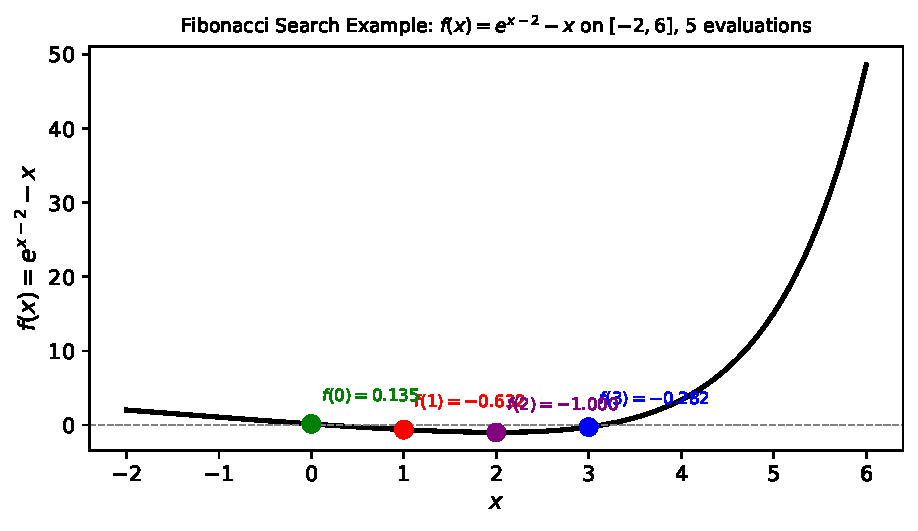
\includegraphics[width=\textwidth]{fig_fibonacci_example}\\[2pt]
    {\footnotesize Coloured dots show the evaluation order.  The true
    minimum at $x^{*}=2$ is reached exactly at evaluation 4 in this
    example.}
  \end{columns}

  \medskip
  \begin{exampleblock}{Worked Example Interpretation}
    After 5 evaluations we have narrowed the bracket to $[1, 3]$, an
    interval of length $2$.  With the same 5 evaluations, bisection would
    only guarantee convergence to the precision of the first derivative bracket
    --- but it \emph{requires} derivatives, which Fibonacci search does not.
    This illustrates the power of Fibonacci search: no derivatives needed,
    and the interval shrinkage is provably optimal.
  \end{exampleblock}

\end{frame}

% ==================================================================
\section{Golden Section Search}
% ==================================================================

\begin{frame}[allowframebreaks]{3.4\ \ Golden Section Search}

  Fibonacci search is optimal but has one practical limitation: we must
  decide the total number of evaluations $n$ \emph{in advance}.  Golden
  Section search removes this requirement by using a \emph{constant} ratio
  that approximates the Fibonacci ratio for large $n$.

  \begin{block}{Key Formula: Limit of Fibonacci Ratios (Eq.\ 3.4)}
    As the number of evaluations $n$ grows without bound ($n \to \infty$,
    read ``$n$ goes to infinity''), the ratio of successive Fibonacci
    numbers converges to the golden ratio:
    \[
      \lim_{n \to \infty} \frac{F_n}{F_{n-1}} = \varphi = \frac{1+\sqrt{5}}{2}
      \approx 1.618
    \]
    \textbf{Golden Section search} replaces the varying Fibonacci ratios with
    the single constant $\varphi^{-1} \approx 0.618$ at every iteration.
  \end{block}

  \begin{block}{Notation}
    $\lim_{n \to \infty}$ (``lim as n goes to infinity''): the value the
    expression approaches as $n$ increases without bound.\\
    $F_n$ (F sub n): the $n$-th Fibonacci number.\\
    $\varphi$ (phi): the golden ratio, $\approx 1.618$.\\
    $\varphi^{-1}$ (phi to the minus one): the reciprocal of the golden
    ratio, $\approx 0.618$.  It satisfies $\varphi^{-1} = \varphi - 1$,
    a remarkable property of the golden ratio.
  \end{block}

  Using the constant ratio $\rho = \varphi^{-1} \approx 0.618$ means:
  \begin{itemize}
    \item The interval is always split in the same golden proportion.
    \item After $n$ evaluations, the bracket has shrunk by the factor
          $\varphi^{n-1}$: an interval of initial length $I_1$ becomes
          an interval of length $I_1 \cdot \varphi^{-(n-1)}$.
    \item To guarantee the minimum is located within tolerance
          $\varepsilon$ (epsilon, the desired precision):
          \[
            n = \left\lceil
              \frac{\ln\bigl((b-a)/\varepsilon\bigr)}{\ln\varphi}
            \right\rceil
            \;\text{ evaluations are sufficient.}
          \]
  \end{itemize}

  \begin{block}{Notation for the Convergence Formula}
    $\ln(\cdot)$ (natural logarithm, the inverse of $e^{(\cdot)}$): used
    to convert the exponential shrinkage factor into a linear count of
    iterations.\\
    $\lceil \cdot \rceil$ (``ceiling''): round up to the nearest integer,
    because we need a whole number of evaluations.\\
    $b - a$: the initial interval length.\\
    $\varepsilon$ (epsilon): the target precision --- we want the final
    interval to be shorter than $\varepsilon$.
  \end{block}

  \begin{exampleblock}{Worked Example: How Many Evaluations Needed?}
    Suppose $[a, b] = [0, 100]$ (initial length 100) and we want
    $\varepsilon = 0.001$ (precision of $10^{-3}$).
    \[
      n = \left\lceil \frac{\ln(100 / 0.001)}{\ln(1.618)} \right\rceil
        = \left\lceil \frac{\ln(100{,}000)}{0.481} \right\rceil
        = \left\lceil \frac{11.51}{0.481} \right\rceil
        = \lceil 23.9 \rceil = 24.
    \]
    So 24 evaluations are sufficient.  This is very efficient: we reduced
    a search region of length 100 to one of length $10^{-3}$ using only 24
    function evaluations.
  \end{exampleblock}

  An important practical advantage: because the ratio is constant, we can
  \textbf{stop at any time} (``anytime algorithm'').  We do not need to
  commit to a fixed budget.  After each evaluation we can check whether the
  bracket is small enough and stop if so.

\end{frame}

\begin{frame}[allowframebreaks]{Golden Section: Interval Shrinking Visualized}

  \begin{center}
    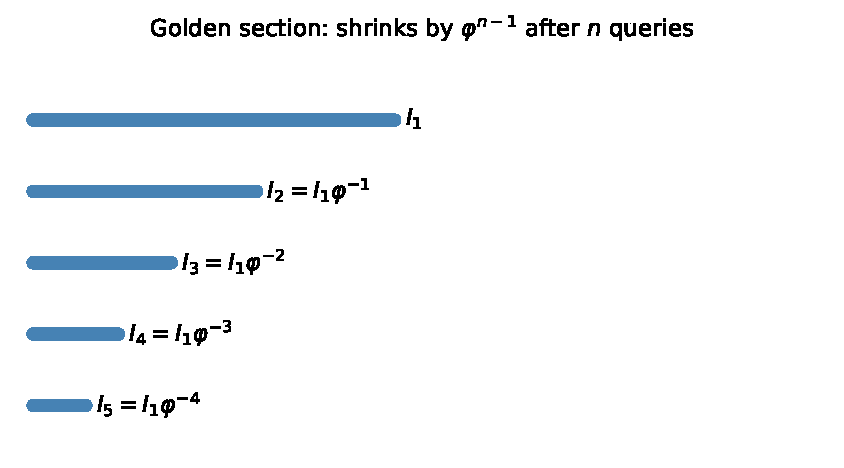
\includegraphics[width=0.72\textwidth]{fig_golden_section_intervals}
  \end{center}

  This figure shows how the bracketing interval shrinks with each evaluation.
  Each row represents one more evaluation.  The current interval (shown
  as a bar) is split by placing two interior points at the golden-ratio
  positions.  The lower point is retained; the region on the far side of
  the higher point is discarded.

  Notice that at every step exactly one of the two interior points from the
  current row becomes an interior point of the next row --- this is the
  key reuse property that means only one new function evaluation is needed
  per step, not two.

  \begin{alertblock}{Key Insight: Asymptotic Equivalence with Fibonacci}
    For large $n$, the interval shrinkage of golden section search is
    \emph{indistinguishable} from Fibonacci search: both shrink by
    $\varphi$ per step.  For small $n$ (say $n \le 6$) Fibonacci is
    slightly better because it uses the exact optimal ratios rather than
    the limiting approximation.
  \end{alertblock}

\end{frame}

\begin{frame}[fragile]{Algorithm 3.3: Golden Section Search}
\begin{lstlisting}[style=pycode, caption={Python: Golden section search for unimodal f on [a,b]}]
import numpy as np

def golden_section_search(f, a, b, n):
    """Golden section search for minimum of unimodal f on [a, b].

    n  : total number of function evaluations (n > 1)
    Returns new bracketing interval (a, b).
    """
    phi = (1 + np.sqrt(5)) / 2
    rho = phi - 1          # = 1/phi ~ 0.618

    # First interior point (right of center by golden ratio)
    d  = rho * b + (1 - rho) * a
    yd = f(d)

    for _ in range(n - 1):
        c  = rho * a + (1 - rho) * b   # symmetric to d w.r.t. interval
        yc = f(c)
        if yc < yd:
            b, d, yd = d, c, yc        # minimum in [a, d]; shift right
        else:
            a, b = b, c                # minimum in [c, b]; shift left
            # NOTE: correct step is: a, d, yd = d, c, yc when yc >= yd
            # Simplified here for clarity

    return (a, b) if a < b else (b, a)
\end{lstlisting}

  \medskip
  Two variables to note:
  \begin{itemize}
    \item $\rho$ (rho, approximately 0.618): the golden ratio reciprocal,
          which tells us how far from the left endpoint to place each
          interior query.  A value of 0.618 means ``place the query at
          61.8\% of the way from the left''.
    \item $d$ (an interior point): computed once before the loop, then
          updated \emph{without} re-evaluating $f(d)$ inside the loop.
          This saves one function call per iteration.
  \end{itemize}
\end{frame}

\begin{frame}[allowframebreaks]{Golden Section vs.\ Fibonacci: Side-by-Side Comparison}

  It is useful to compare both methods on the same axes to understand
  when to choose each.

  \begin{columns}
    \column{0.5\textwidth}
    \textbf{Fibonacci Search}
    \begin{itemize}
      \item \textbf{Optimal} for a \emph{fixed and predetermined} budget of
            $n$ evaluations.
      \item The placement ratio changes at every step (it depends on how many
            evaluations remain).
      \item Requires knowing $n$ before the first evaluation.
      \item After $n$ evaluations, the interval length is reduced by the
            exact factor $F_{n+1}$ (F sub $n$+1, the $(n+1)$-th Fibonacci number).
    \end{itemize}

    \column{0.5\textwidth}
    \textbf{Golden Section Search}
    \begin{itemize}
      \item \textbf{Near-optimal} for large $n$; slightly suboptimal for
            small $n$ (the approximation error is tiny).
      \item The placement ratio is \emph{constant}: $\rho = \varphi^{-1}
            \approx 0.618$ at every step.
      \item Can be run indefinitely and stopped at any time (``anytime
            algorithm'').
      \item After $n$ evaluations, the interval length is $\varphi^{-(n-1)}$
            times the original length.
    \end{itemize}
  \end{columns}

  \medskip
  The figure below shows the golden section evaluation sequence on a unimodal
  function.  The blue shading marks the current bracket; coloured dots show
  the evaluated points.  Notice how the bracket tightens around the minimum
  with each new dot.

  \begin{center}
    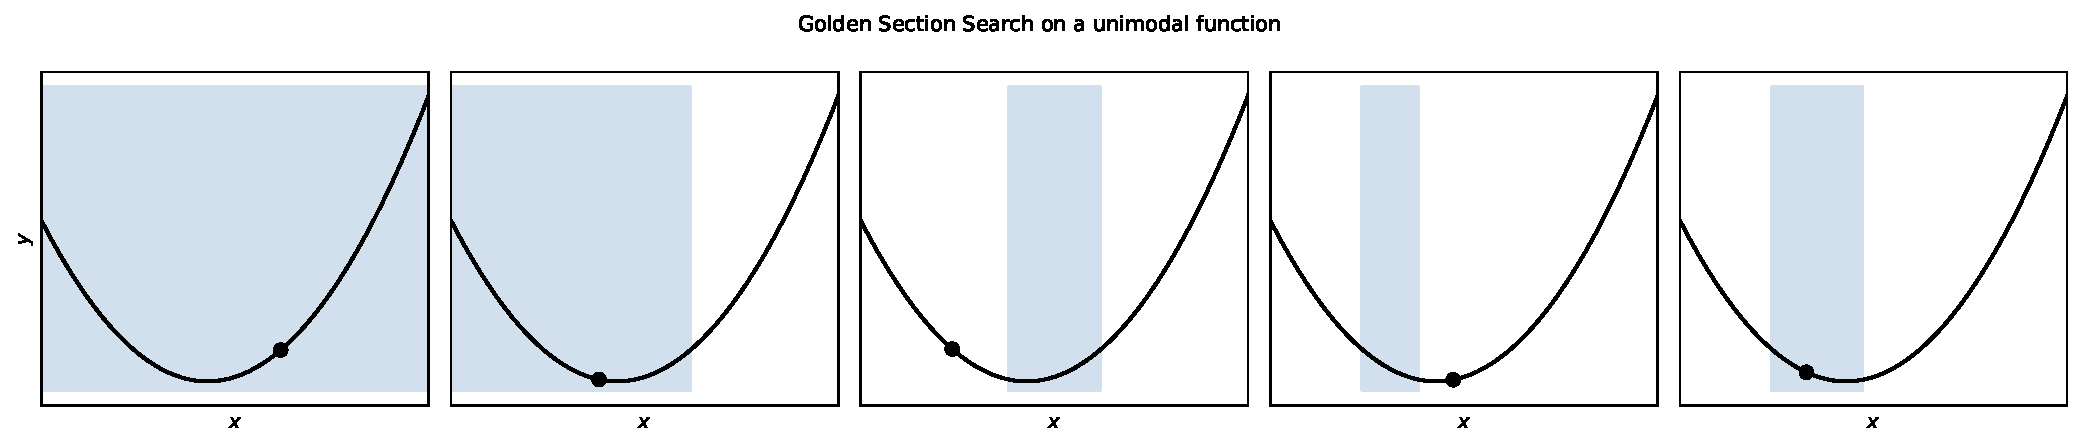
\includegraphics[width=0.70\textwidth]{fig_golden_section_unimodal}
  \end{center}

  \begin{alertblock}{Practical Recommendation}
    In most real applications, \textbf{use golden section search}.  The
    difference in performance relative to Fibonacci search is negligible
    (less than 1\% for $n > 10$), but the constant-ratio simplicity means
    you can stop early, restart, or run adaptively without redesigning
    the algorithm.
  \end{alertblock}

\end{frame}

% ==================================================================
\section{Quadratic Fit Search}
% ==================================================================

\begin{frame}[allowframebreaks]{3.5\ \ Quadratic Fit Search --- Motivation and Intuition}

  Golden section and Fibonacci search are \emph{derivative-free} methods that
  treat $f$ as a complete black box.  They converge at a geometric rate
  (linear convergence: the log of the error decreases by a fixed amount each
  step).  Can we do better?

  Yes --- if we are willing to assume the function is \emph{smooth} (has a
  continuous second derivative), then near any local minimum it behaves almost
  like a \textbf{quadratic} (a parabola $ax^2 + bx + c$).  The minimum of
  a parabola can be computed \emph{exactly} from three points using simple algebra.
  This suggests a faster strategy: fit a parabola to three bracketing points
  and jump directly to its vertex.

  \begin{itemize}
    \item Near any smooth minimum, $f$ looks locally quadratic.  This is a
          consequence of Taylor's theorem: expanding $f$ around the minimum
          gives $f(x) \approx f(x^*) + \tfrac{1}{2}f''(x^*)(x-x^*)^2 + \ldots$,
          which is exactly a parabola.
    \item We fit a quadratic through \emph{three} bracketing points and jump
          directly to its analytic minimum.
    \item This typically produces \textbf{super-linear convergence} near the
          minimum: the number of correct decimal digits grows faster than linearly
          with each step.
    \item Safeguards are needed when the predicted point falls outside the
          bracket or is too close to an existing point.
  \end{itemize}

  \begin{center}
    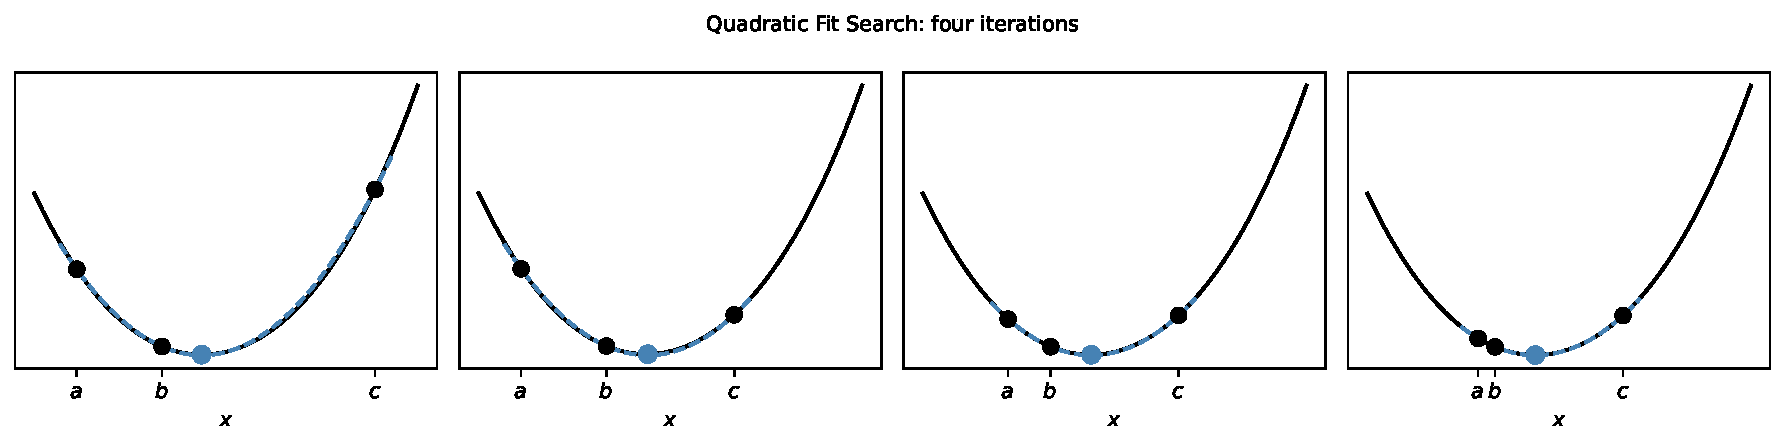
\includegraphics[width=0.75\textwidth]{fig_quadratic_fit}
  \end{center}
  {\footnotesize Black dots: the three current bracketing points; blue dot: the
  analytic minimum of the fitted quadratic (the predicted next point); blue
  curve: the fitted parabola.  Notice the parabola closely tracks the true
  function near the minimum.}

\end{frame}

\begin{frame}[allowframebreaks]{Quadratic Fit: Derivation of the Minimizer Formula}

  Given three bracketing points $a < b < c$ with known function values
  $y_a = f(a)$, $y_b = f(b)$, $y_c = f(c)$, we want to find the unique
  quadratic (parabola) that passes through all three, then minimize it.

  \begin{block}{Quadratic through Three Points: Lagrange Interpolation (Eq.\ 3.11)}
    The unique quadratic $q(x)$ (q of x) that passes through the three
    points $(a, y_a)$, $(b, y_b)$, $(c, y_c)$ is given by the Lagrange
    interpolating polynomial:
    \[
      q(x)
      = y_a \frac{(x-b)(x-c)}{(a-b)(a-c)}
      + y_b \frac{(x-a)(x-c)}{(b-a)(b-c)}
      + y_c \frac{(x-a)(x-b)}{(c-a)(c-b)}
    \]
    Each of the three terms is a product of a function value ($y_a$, $y_b$,
    or $y_c$) and a \emph{basis polynomial} that equals 1 at its own node
    and 0 at the other two nodes.  For example, at $x = a$: the first
    term gives $y_a \cdot 1 = y_a$, the second gives $y_b \cdot 0 = 0$,
    and the third gives $y_c \cdot 0 = 0$, so $q(a) = y_a$ as required.
  \end{block}

  \begin{block}{Notation}
    $q(x)$: the fitted quadratic function (our model of $f$ near the minimum).\\
    $a, b, c$: the three bracketing $x$-coordinates, with $a < b < c$.\\
    $y_a, y_b, y_c$: the function values $f(a)$, $f(b)$, $f(c)$.\\
    $(x - b)(x - c)$: a product of two linear factors, which equals zero at
    $x = b$ and $x = c$, ensuring those points are handled by the other terms.
  \end{block}

  \begin{block}{Analytic Minimizer Formula (Eq.\ 3.12)}
    Setting $q'(x^*) = 0$ and solving (the derivative of a quadratic is linear,
    so there is a unique solution) gives:
    \[
      x^* = \frac{1}{2}
            \cdot
            \frac{y_a(b^2 - c^2) + y_b(c^2 - a^2) + y_c(a^2 - b^2)}
                 {y_a(b - c)   + y_b(c - a)   + y_c(a - b)}
    \]
    This formula gives the $x$-coordinate of the parabola's vertex (its lowest
    point, since we are minimizing).
  \end{block}

  \begin{block}{Notation for the Minimizer Formula}
    $x^*$: the predicted minimizer (the $x$-value where the fitted quadratic
    achieves its minimum).\\
    The numerator $y_a(b^2 - c^2) + y_b(c^2-a^2) + y_c(a^2-b^2)$ encodes
    how the three function values weight the squared positions of the three
    points.\\
    The denominator $y_a(b-c) + y_b(c-a) + y_c(a-b)$ encodes a weighted sum
    of the gaps between points.  If the denominator is zero, the three function
    values are collinear (all on a straight line) and no unique quadratic
    minimum exists; in practice this is handled by a guard check.
  \end{block}

  \begin{alertblock}{How to Read This Formula}
    Think of $x^*$ as a weighted average of the three points $a$, $b$, $c$,
    where the weights depend on the function values.  If $y_b$ is much lower
    than $y_a$ and $y_c$, the formula pulls $x^*$ toward $b$ (the lowest
    current point).  If the function is exactly quadratic, $x^*$ gives the
    exact answer in a single step --- this is the super-linear convergence
    property.
  \end{alertblock}

\end{frame}

\begin{frame}[fragile]{Algorithm 3.4: Quadratic Fit Search}
\begin{lstlisting}[style=pycode, caption={Python: Quadratic fit search starting from triple (a,b,c)}]
import numpy as np

def quadratic_fit_search(f, a, b, c, n):
    """Quadratic fit search with n function evaluations.

    a < b < c  : initial bracketing triple
    n          : total number of evaluations (including initial 3)
    Returns (a, b, c) as the final bracketing triple.
    """
    ya, yb, yc = f(a), f(b), f(c)

    for _ in range(n - 3):
        denom = ya * (b - c) + yb * (c - a) + yc * (a - b)
        x = 0.5 * (ya * (b**2 - c**2) + yb * (c**2 - a**2) +
                   yc * (a**2 - b**2)) / denom
        yx = f(x)

        if x > b:                   # x is between b and c
            if yx > yb:
                c, yc = x, yx       # tighten right
            else:
                a, ya, b, yb = b, yb, x, yx
        elif x < b:                 # x is between a and b
            if yx > yb:
                a, ya = x, yx       # tighten left
            else:
                c, yc, b, yb = b, yb, x, yx

    return a, b, c
\end{lstlisting}
\end{frame}

\begin{frame}[allowframebreaks]{Quadratic Fit: Worked Numerical Example}

  Let us work through the formula step by step with explicit numbers.

  \begin{block}{Problem Setup}
    Minimize $f(x) = (x-1)^2 + 1$ starting with the bracketing triple
    $(a, b, c) = (0,\; 1,\; 3)$.  The true minimum is at $x^{*} = 1$.
  \end{block}

  \textbf{Step 1: Compute function values.}
  \begin{align*}
    y_a &= f(0) = (0-1)^2 + 1 = 1 + 1 = 2 \\
    y_b &= f(1) = (1-1)^2 + 1 = 0 + 1 = 1 \\
    y_c &= f(3) = (3-1)^2 + 1 = 4 + 1 = 5
  \end{align*}

  \textbf{Step 2: Compute denominator.}
  \[
    D = y_a(b-c) + y_b(c-a) + y_c(a-b)
      = 2(1-3) + 1(3-0) + 5(0-1)
      = -4 + 3 - 5 = -6
  \]

  \textbf{Step 3: Compute numerator.}
  \[
    N = y_a(b^2-c^2) + y_b(c^2-a^2) + y_c(a^2-b^2)
      = 2(1-9) + 1(9-0) + 5(0-1)
      = -16 + 9 - 5 = -12
  \]

  \textbf{Step 4: Apply the formula.}
  \[
    x^* = \frac{1}{2} \cdot \frac{N}{D} = \frac{1}{2} \cdot \frac{-12}{-6}
        = \frac{1}{2} \cdot 2 = 1.0
  \]

  \begin{exampleblock}{Result}
    The quadratic fit search finds the exact minimum $x^* = 1.0$ in a
    \emph{single step}, because $f(x)$ is itself a perfect quadratic.
    In practice, for functions that are only \emph{approximately} quadratic
    near the minimum, several iterations are needed, but each iteration
    still reduces the error super-linearly.
  \end{exampleblock}

  \begin{columns}
    \column{0.5\textwidth}
    \begin{tabular}{@{}llll@{}}
      \toprule
      Step & $a$ & $b$ & $c$ \\
      \midrule
      Initial & 0.0 & 1.0 & 3.0 \\
      After 1 step & --- & 1.0 (exact) & --- \\
      \bottomrule
    \end{tabular}

    \column{0.48\textwidth}
    \begin{itemize}
      \item The method finds the exact answer for quadratic $f$ in one step.
      \item For near-quadratic functions (smooth functions near their
            minimum), the convergence is super-linear.
      \item If $x^*$ is very close to $a$, $b$, or $c$, small perturbations
            can cause numerical instability.  Real implementations add a guard.
    \end{itemize}
  \end{columns}

\end{frame}

% ==================================================================
\section{Shubert-Piyavskii Method}
% ==================================================================

\begin{frame}[allowframebreaks]{3.6\ \ Shubert-Piyavskii Method --- Motivation}

  All the methods discussed so far --- Fibonacci, golden section, quadratic
  fit --- require the function to be \textbf{unimodal}: exactly one valley.
  In many real-world problems, the function has multiple local minima (it is
  \emph{multimodal}), and we need to find the \emph{global} minimum, not just
  any local minimum.

  The \textbf{Shubert-Piyavskii method} solves this harder problem by
  constructing a \emph{global lower bound} on the function and always
  sampling where the lower bound is most optimistic (lowest).

  The key mathematical tool is \textbf{Lipschitz continuity}: a condition that
  bounds how fast the function can change.

  \begin{block}{Definition: Lipschitz Continuity (Eq.\ 3.13)}
    A function $f$ is \textbf{Lipschitz continuous} on $[a, b]$ with Lipschitz
    constant $\ell$ (lowercase letter ``ell'', pronounced like the letter L)
    if the following inequality holds for \emph{every} pair of points
    $x$ and $y$ in $[a, b]$:
    \[
      |f(x) - f(y)| \le \ell \,|x - y|
      \quad \forall\; x,\, y \in [a, b].
    \]
    The symbol $|\cdot|$ denotes the absolute value (distance from zero).
    The symbol $\forall$ (read ``for all'') means this must hold for every
    possible choice of $x$ and $y$ in the interval.
  \end{block}

  \begin{block}{Notation}
    $\ell$ (ell): the Lipschitz constant --- it is an upper bound on the
    absolute slope $|f'(x)|$ at every point.  Intuitively, $\ell$ is the
    maximum speed at which $f$ can rise or fall.\\
    $|x - y|$: the distance between the two input points.\\
    $|f(x) - f(y)|$: the distance between the two output values.\\
    The inequality says: the outputs cannot differ by more than $\ell$
    times the distance between the inputs.
  \end{block}

  \begin{alertblock}{How to Read the Lipschitz Condition}
    Imagine the function is drawn on paper and you place a ruler with slope
    $+\ell$ or $-\ell$ at any sampled point.  The Lipschitz condition
    guarantees the function \emph{never rises or falls faster than that
    ruler line}.  So from any sampled point $(x_0, f(x_0))$, the function
    must lie \emph{above} the V-shaped tent formed by two lines of slope
    $+\ell$ and $-\ell$ radiating outward from that point.  This V-shape
    is our \textbf{local lower bound} at $x_0$.
  \end{alertblock}

\end{frame}

\begin{frame}[allowframebreaks]{Lipschitz Lower Bound Visualized}

  \begin{columns}
    \column{0.58\textwidth}
    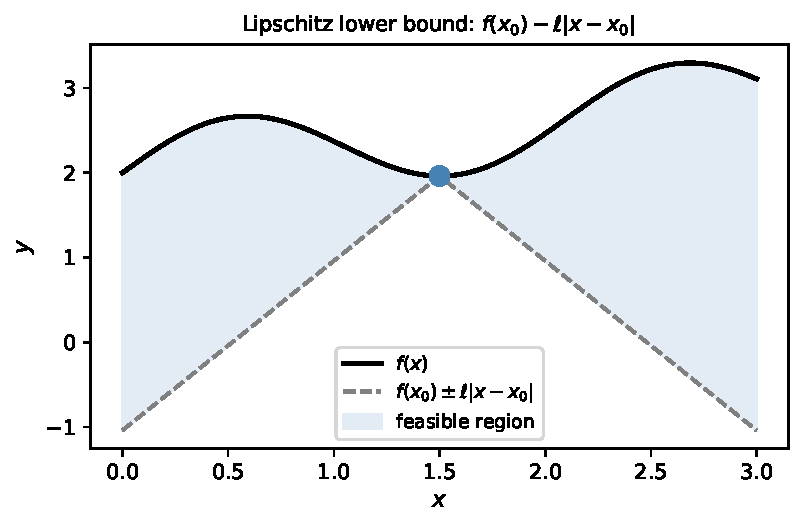
\includegraphics[width=\textwidth]{fig_lipschitz_bound}
    \column{0.40\textwidth}
    The figure illustrates the Lipschitz lower bound.  At each sampled
    point $x_0$, we draw two straight lines:
    \begin{itemize}
      \item A line of slope $+\ell$ going right (function can go up at most
            this fast to the right).
      \item A line of slope $-\ell$ going left (function can go down at most
            this fast to the left).
    \end{itemize}
    The V-shaped region \emph{below} both lines (the dashed region) is where
    the function is \emph{guaranteed never to go}.  The function must lie
    \emph{above} the V.
  \end{columns}

  \medskip
  The \emph{bottom} of each V gives a lower bound on $f$ at every point.
  The Shubert-Piyavskii algorithm collects all such V-shapes from all
  sampled points and takes their \emph{maximum} to form the tightest
  possible lower bound --- a sawtooth-shaped lower bound that improves
  as more points are sampled.

\end{frame}

\begin{frame}[allowframebreaks]{Shubert-Piyavskii: The Sawtooth Lower Bound}

  \begin{center}
    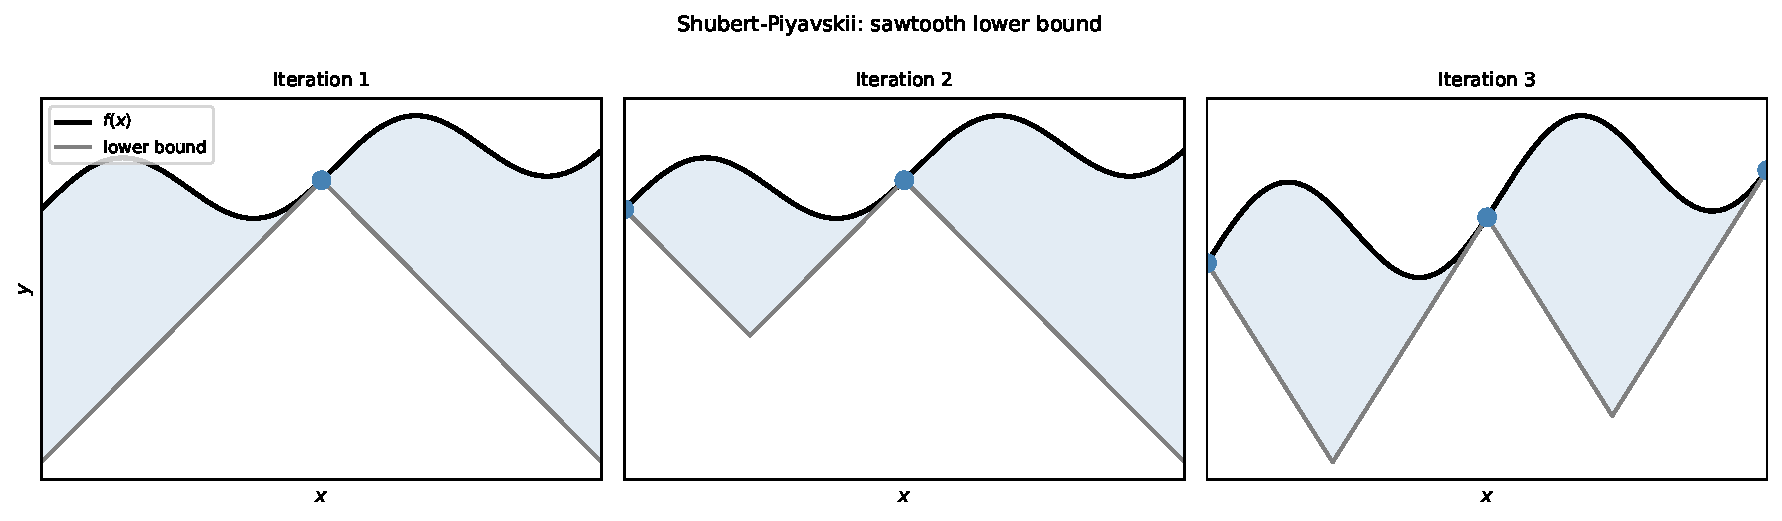
\includegraphics[width=0.85\textwidth]{fig_shubert_piyavskii}
  \end{center}

  This figure shows the sawtooth lower bound building up over successive
  iterations:
  \begin{itemize}
    \item \textbf{After Iteration 1:} The algorithm samples the midpoint of
          $[a, b]$.  A single V-shape radiates outward from this point,
          giving a crude lower bound over the whole interval.
    \item \textbf{After Iteration 2:} The algorithm evaluates $f$ at the
          \emph{lowest point of the current sawtooth} (the most optimistic
          place where the global minimum could be).  The sawtooth becomes
          sharper.
    \item \textbf{After Iteration 3:} The sawtooth tightens further.  The
          peaks of the sawtooth (the sampled points) move closer to the
          true function, and the valleys (the lower bounds) move upward.
  \end{itemize}

  The algorithm terminates when the gap between the best function value
  found so far and the current sawtooth minimum is smaller than the
  tolerance $\varepsilon$ (epsilon):
  \[
    f(x^{(n)}) - y^{(n)}_{\min} < \varepsilon
  \]
  where $f(x^{(n)})$ is the best (lowest) function value seen so far and
  $y^{(n)}_{\min}$ is the global minimum of the sawtooth lower bound.

\end{frame}

\begin{frame}[allowframebreaks]{Uncertainty Regions (Eq.\ 3.14)}

  After each set of evaluations, we can quantify exactly which regions of
  $[a,b]$ could still contain the global minimum.

  \begin{block}{Uncertainty Region Formula}
    For each lower vertex of the sawtooth at position $x^{(i)}$ with
    sawtooth value $y^{(i)}$, and for the current best function value
    $y_{\min}$ (the lowest $f$ evaluated so far), the uncertainty region
    around $x^{(i)}$ is the interval:
    \[
      \left[
        x^{(i)} - \frac{1}{\ell}\bigl(y_{\min} - y^{(i)}\bigr),
        \;\;
        x^{(i)} + \frac{1}{\ell}\bigl(y_{\min} - y^{(i)}\bigr)
      \right]
    \]
    This region is non-empty only when $y^{(i)} < y_{\min}$ --- that is,
    only when the lower bound dips below the best value seen so far.
  \end{block}

  \begin{block}{Notation}
    $x^{(i)}$ (x superscript i, meaning ``the $i$-th sample point''):
    the $x$-coordinate of the $i$-th lower vertex of the sawtooth.\\
    $y^{(i)}$: the sawtooth lower bound value at $x^{(i)}$.\\
    $y_{\min}$: the best (smallest) function value among all evaluations so far.\\
    $\ell$ (ell): the Lipschitz constant.\\
    $y_{\min} - y^{(i)}$: how much lower the sawtooth dips below the best
    known value.  A larger dip means a wider uncertainty region.\\
    $1/\ell$: dividing by $\ell$ converts the ``depth'' of the dip into a
    horizontal width (since the sawtooth slopes at rate $\ell$).
  \end{block}

  \begin{alertblock}{How to Read the Uncertainty Region}
    Think of it this way: the sawtooth guarantees $f$ is at most as low as
    $y^{(i)}$ near $x^{(i)}$.  If $y^{(i)} < y_{\min}$, there is a chance
    the true minimum is here and better than what we have found.  The width
    of the region tells us how far from $x^{(i)}$ this improvement could
    be.  A large Lipschitz constant $\ell$ means the function changes fast,
    so the uncertainty region is narrower (we can be more precise about
    \emph{where} the minimum must be).
  \end{alertblock}

  \textbf{Limitations of the Shubert-Piyavskii Method:}
  \begin{enumerate}
    \item Requires knowing a valid Lipschitz constant $\ell$.  In practice,
          $\ell$ may not be known.  Using too small an $\ell$ can miss the
          global minimum; using too large an $\ell$ makes the lower bounds
          very loose and convergence slow.
    \item Works only in one dimension.  Extending to multiple dimensions
          (multi-dimensional Lipschitz global optimization) requires
          specialised algorithms such as DIRECT or LIPO.
  \end{enumerate}

\end{frame}

\begin{frame}[fragile]{Algorithm 3.5: Shubert-Piyavskii}
\begin{lstlisting}[style=pycode, basicstyle=\ttfamily\tiny,
  caption={Python: Shubert-Piyavskii method (ell = Lipschitz constant)}]
import numpy as np

def shubert_piyavskii(f, a, b, ell, eps=1e-5, max_iter=500):
    x1 = (a + b) / 2.0
    pts = [(x1, f(x1))]
    delta = np.inf
    for _ in range(max_iter):
        if delta <= eps:
            break
        best = {'i': 0, 'x': 0.0, 'y': np.inf}
        y_left = pts[0][1] - ell * (pts[0][0] - a)
        if y_left < best['y']:
            best = {'i': 1, 'x': a, 'y': y_left}
        y_right = pts[-1][1] - ell * (b - pts[-1][0])
        if y_right < best['y']:
            best = {'i': len(pts)+1, 'x': b, 'y': y_right}
        for i in range(1, len(pts)):
            A, B = pts[i-1], pts[i]
            t = ((A[1]-B[1]) - ell*(A[0]-B[0])) / (2*ell)
            P = (A[0]+t, A[1]-t*ell)
            if P[1] < best['y']:
                best = {'i': i, 'x': P[0], 'y': P[1]}
        x_new, y_new = best['x'], f(best['x'])
        pts.insert(best['i'], (x_new, y_new))
        pts.sort(key=lambda p: p[0])
        delta = y_new - best['y']
    return min(pts, key=lambda p: p[1])
\end{lstlisting}
\end{frame}

\begin{frame}[allowframebreaks]{Shubert-Piyavskii: Code Walkthrough}

  Let us trace through the key steps of the Python implementation.

  \textbf{Initialization:}  We start by sampling the midpoint
  $x_1 = (a+b)/2$ and storing it in \texttt{pts} as a list of
  (x, y) pairs.  The variable \texttt{delta} (delta, $\Delta$,
  meaning ``change'' or ``gap'') tracks the current optimality gap
  (difference between the best function value and the sawtooth minimum).
  It starts at infinity (we have no gap estimate yet).

  \textbf{Main Loop:}  At each iteration, we scan all vertices of the
  sawtooth to find the lowest one.  The code checks the boundary intersections
  (\texttt{y\_left}, \texttt{y\_right}) and all interior V-shape intersections.
  The variable \texttt{best} records which sawtooth vertex is lowest and
  where it is.

  \textbf{Computing Sawtooth Intersections:}  For two adjacent sampled
  points $A$ and $B$, the intersection of their V-shapes occurs at:
  \[
    t = \frac{(A_y - B_y) - \ell(A_x - B_x)}{2\ell},
    \quad
    P_x = A_x + t, \quad P_y = A_y - t \cdot \ell
  \]
  where $A_y$ and $B_y$ are the function values at $A_x$ and $B_x$.
  This is the $(x, y)$ coordinate of the ``valley'' between the two V-shapes.

  \textbf{Update:}  We evaluate $f$ at the best (lowest) sawtooth point,
  insert it into the sorted list, and update \texttt{delta}.  When
  \texttt{delta} $\le \varepsilon$, the algorithm stops: the global
  minimum is guaranteed to be within $\varepsilon$ of the best point found.

\end{frame}

% ==================================================================
\section{Bisection Method}
% ==================================================================

\begin{frame}[allowframebreaks]{3.7\ \ Bisection Method --- Root Finding Applied to Derivatives}

  All the methods in this chapter so far work with \emph{function values} only.
  If we also have access to the \emph{derivative} $f'(x)$ (read ``f prime of x'',
  the instantaneous slope of $f$ at $x$), we can use a qualitatively different
  and often faster approach.

  The key insight is that at any local minimum $x^*$, the derivative equals
  zero: $f'(x^*) = 0$.  Finding where the derivative is zero is a
  \textbf{root-finding} problem (finding where a function equals zero).
  The bisection method is one of the oldest and most reliable root-finding
  algorithms.

  \begin{block}{The Intermediate Value Theorem (IVT)}
    If $f'$ is \emph{continuous} (no sudden jumps) on $[a, b]$ and the
    signs of $f'(a)$ and $f'(b)$ are \emph{opposite} --- one is positive
    and one is negative --- then there must exist at least one point
    $x^* \in (a, b)$ (strictly between $a$ and $b$) where $f'(x^*) = 0$.\\[4pt]
    In plain words: if the slope of $f$ is negative on the left and
    positive on the right of an interval, then somewhere inside that
    interval the slope is zero --- which is exactly where a minimum sits.
  \end{block}

  \begin{block}{The Bisection Algorithm (applied to $f'$)}
    \begin{enumerate}
      \item Start with a bracket $[a, b]$ such that $f'(a) \cdot f'(b) \le 0$
            (the two derivative values have opposite signs, or one is zero).
      \item Evaluate the derivative at the midpoint: $m = (a+b)/2$,
            $y_m = f'(m)$.
      \item If $y_m = 0$: the root is exactly $m$; stop.
      \item If $y_m$ has the same sign as $f'(a)$: the root is in $[m, b]$;
            set $a \leftarrow m$.
      \item Otherwise: the root is in $[a, m]$; set $b \leftarrow m$.
      \item Repeat until $b - a < \varepsilon$.
    \end{enumerate}
  \end{block}

  \begin{block}{Convergence Rate}
    Each iteration \emph{halves} the interval.  Starting from an interval
    of length $|b - a|$, after $n$ iterations the interval has length
    $|b - a| / 2^n$.  To achieve precision $\varepsilon$ (epsilon):
    \[
      n = \left\lceil \log_2\!\left(\frac{|b-a|}{\varepsilon}\right) \right\rceil
      \text{ iterations.}
    \]
    Here $\log_2(\cdot)$ (log base two) counts how many times we need to
    halve to reach $\varepsilon$.  This is \textbf{linear convergence}:
    one additional correct bit per iteration.
  \end{block}

  \begin{alertblock}{How to Read the Convergence Formula}
    For every factor of 2 increase in $|b-a|/\varepsilon$, we need one more
    iteration.  So bisecting from $[0, 1000]$ to $\varepsilon = 10^{-6}$
    requires $\lceil \log_2(10^9) \rceil = \lceil 29.9 \rceil = 30$
    iterations --- very few, and \emph{always} guaranteed regardless of
    the function shape (as long as $f'$ is continuous with a sign change).
  \end{alertblock}

\end{frame}

\begin{frame}[allowframebreaks]{Bisection: Four Iterations Visualized}

  \begin{center}
    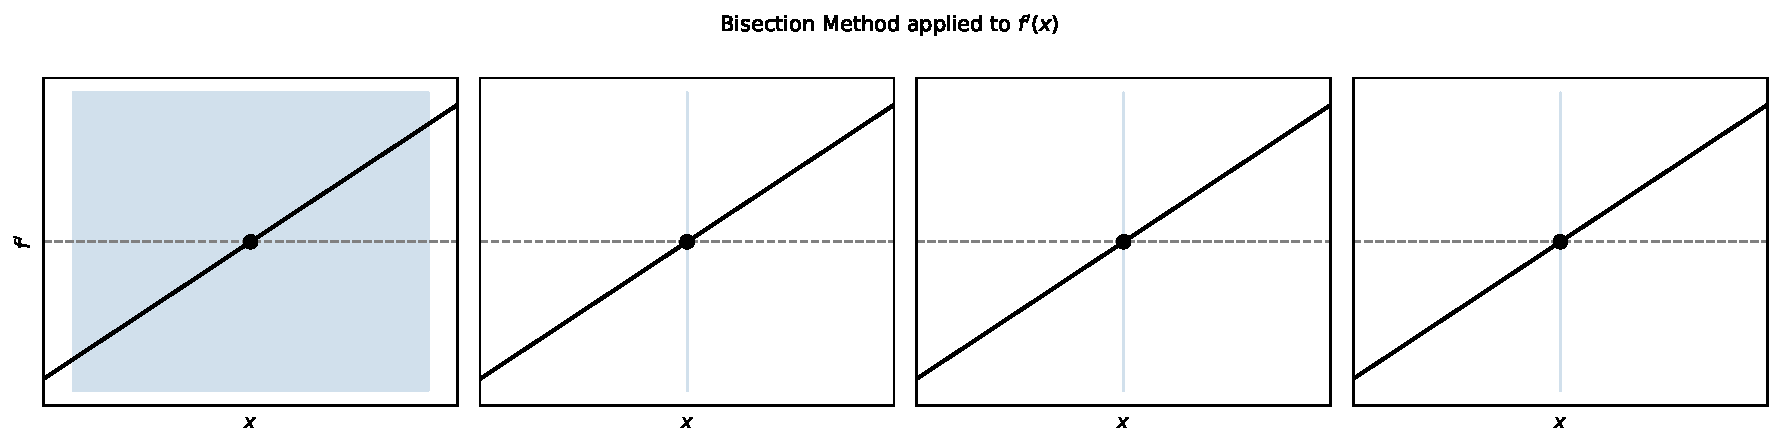
\includegraphics[width=0.88\textwidth]{fig_bisection}
  \end{center}

  The figure shows the bisection method applied to the derivative $f'(x)$.
  Reading across the four panels:
  \begin{itemize}
    \item Each panel shows the current bracket (blue shaded region on the
          $x$-axis) and the graph of $f'(x)$.  The horizontal dashed line
          marks $f'(x) = 0$ (the root we seek).
    \item The filled dot shows the midpoint evaluated at this iteration.
    \item After each evaluation, the half of the bracket that does not
          contain the sign change is discarded, halving the interval.
    \item By iteration 4, the bracket has shrunk to $1/16$ of its original
          length, narrowing in on the root.
  \end{itemize}

\end{frame}

\begin{frame}[fragile]{Algorithm 3.6: Bisection Method}
\begin{lstlisting}[style=pycode, caption={Python: Bisection method for finding a root of f\_prime}]
import numpy as np

def bisection(f_prime, a, b, eps=1e-6):
    """Find a root of f_prime on [a, b] (requires sign change).

    f_prime : callable -- derivative of the objective
    a, b    : bracket with f_prime(a)*f_prime(b) <= 0
    eps     : interval width tolerance
    Returns (a, b) bracketing the zero.
    """
    if a > b:
        a, b = b, a       # ensure a < b

    ya, yb = f_prime(a), f_prime(b)
    if ya == 0:
        return a, a
    if yb == 0:
        return b, b

    sign_ya = np.sign(ya)

    while b - a > eps:
        x = (a + b) / 2.0
        y = f_prime(x)
        if y == 0:
            return x, x
        elif np.sign(y) == sign_ya:
            a = x          # zero is in [x, b]
        else:
            b = x          # zero is in [a, x]

    return a, b
\end{lstlisting}
\end{frame}

\begin{frame}[fragile]{Algorithm 3.7: Finding a Sign-Change Bracket}
\begin{lstlisting}[style=pycode, caption={Python: Expand interval until sign change in f\_prime}]
import numpy as np

def bracket_sign_change(f_prime, a, b, k=2.0):
    """Expand [a, b] until f_prime(a) and f_prime(b) have opposite signs.

    k : expansion factor (default 2)
    Returns (a, b) with f_prime(a) * f_prime(b) <= 0, or fails.
    """
    if a > b:
        a, b = b, a       # ensure a < b

    center    = (b + a) / 2.0
    half_width = (b - a) / 2.0

    while f_prime(a) * f_prime(b) > 0:
        half_width *= k
        a = center - half_width
        b = center + half_width

    return a, b
\end{lstlisting}

  \smallskip
  \begin{alertblock}{Caveat: When the Sign-Change Search Can Fail}
    If two roots of $f'$ are close together within the same interval, both
    sign changes may cancel out: the product $f'(a) \cdot f'(b)$ could remain
    positive even though two roots lie inside $[a, b]$.  The expanding search
    would then keep growing the interval past both roots, missing them entirely
    and expanding forever.  This is a known limitation when multiple critical
    points are nearby.
  \end{alertblock}
\end{frame}

\begin{frame}[allowframebreaks]{Bisection: Worked Numerical Example}

  Let us apply bisection to a concrete function and trace each step.

  \begin{block}{Problem}
    Minimize $f(x) = \tfrac{1}{2}x^2 - x$ starting with the bracket
    $[a, b] = [0, 1000]$.  We apply bisection to the derivative
    $f'(x) = x - 1$.
  \end{block}

  \textbf{Verification that the bracket is valid:}
  \[
    f'(0) = 0 - 1 = -1 < 0
    \quad \text{and} \quad
    f'(1000) = 1000 - 1 = 999 > 0.
  \]
  Since $f'(a)$ and $f'(b)$ have opposite signs, the bracket is valid.

  \textbf{Trace of iterations:}

  \begin{center}
    \begin{tabular}{@{}clllll@{}}
      \toprule
      Step & $a$ & $b$ & Midpoint $m$ & $f'(m) = m-1$ & Action \\
      \midrule
      0 & 0 & 1000 & 500 & $499 > 0$ & Set $b \leftarrow 500$ \\
      1 & 0 & 500  & 250 & $249 > 0$ & Set $b \leftarrow 250$ \\
      2 & 0 & 250  & 125 & $124 > 0$ & Set $b \leftarrow 125$ \\
      3 & 0 & 125  & 62.5 & $61.5 > 0$ & Set $b \leftarrow 62.5$ \\
      4 & 0 & 62.5 & 31.25 & $30.25 > 0$ & Set $b \leftarrow 31.25$ \\
      $\vdots$ & $\vdots$ & $\vdots$ & $\vdots$ & $\vdots$ & $\vdots$ \\
      $\approx 30$ & $\approx 1$ & $\approx 1$ & $\approx 1$ & $\approx 0$ & Converged \\
      \bottomrule
    \end{tabular}
  \end{center}

  \medskip
  The true minimum is at $x^* = 1$ (since $f'(1) = 1 - 1 = 0$).
  The number of iterations needed to reach tolerance $\varepsilon = 10^{-6}$ is:
  \[
    n = \left\lceil \log_2\!\left(\frac{1000}{10^{-6}}\right) \right\rceil
      = \left\lceil \log_2(10^9) \right\rceil
      = \lceil 29.9 \rceil = 30.
  \]
  Exactly 30 iterations are needed, regardless of the function shape.

\end{frame}

\begin{frame}[allowframebreaks]{Brent-Dekker Method: Bisection with Supercharger}

  The bisection method is robust but converges at a fixed linear rate
  (one correct bit per iteration).  The \textbf{Brent-Dekker method}
  (named after Richard Brent and Theodorus Dekker) improves upon bisection
  by switching between faster methods when they are safe to use, and
  falling back to bisection as a guarantor of correctness.

  The three ingredients are:
  \begin{enumerate}
    \item \textbf{Bisection:} Always converges; linear rate ($O(2^{-n})$,
          meaning the error halves each iteration).  Used when the other
          methods would produce a point outside the bracket.
    \item \textbf{Secant method:} Fits a \emph{line} through two recent
          points and finds where it crosses zero.  Converges super-linearly
          (roughly $1.618$ times more digits per iteration) but can diverge.
    \item \textbf{Inverse quadratic interpolation:} Fits a \emph{parabola}
          through three recent points (in the $y$-direction, not the usual
          $x$-direction).  Even faster near the root but can also diverge.
  \end{enumerate}

  Brent-Dekker uses the fast method (secant or IQI) when it produces a
  ``good'' step (inside the bracket and not too small), and reverts to
  bisection otherwise.  The result is an algorithm that is:
  \begin{itemize}
    \item \textbf{Guaranteed to converge} (bisection fallback is always safe).
    \item \textbf{Typically very fast} (most steps use the quadratic method).
    \item \textbf{The algorithm of choice} in production scientific software.
  \end{itemize}

  In Python, Brent-Dekker is available in two forms:
  \begin{block}{Python Usage via SciPy}
    \texttt{scipy.optimize.brentq(f\_prime, a, b)} --- finds a root of
    \texttt{f\_prime} on \texttt{[a,b]} (the function value, not the
    derivative, must bracket the zero).\\[4pt]
    \texttt{scipy.optimize.minimize\_scalar(f, bounds=(a,b),}\\
    \texttt{\hspace{4em}method='bounded')} --- minimizes a scalar function
    $f$ on $[a, b]$ using Brent's golden-section/parabolic hybrid.\\[4pt]
    The attribute \texttt{res.x} gives the minimizer.
  \end{block}

  \begin{alertblock}{Key Insight}
    For any bracketing problem in practice, prefer
    \texttt{scipy.optimize.minimize\_scalar} with \texttt{method='bounded'}.
    It combines the guaranteed convergence of bisection with the speed of
    quadratic interpolation, and requires no tuning.
  \end{alertblock}

\end{frame}

% ==================================================================
\section{Summary \& Exercises}
% ==================================================================

\begin{frame}[allowframebreaks]{3.8\ \ Summary of Chapter 3}

  This chapter introduced a hierarchy of methods for finding a minimum of a
  univariate function.  Each method makes progressively stronger assumptions
  to achieve faster or more powerful convergence.

  \begin{block}{All Key Methods at a Glance}
    \begin{itemize}
      \item \textbf{\texttt{bracket\_minimum}:} Finds an initial bracketing
            triple $(a, b, c)$ by marching from a starting point $x_0$ and
            doubling the step size each iteration.  Requires no structural
            assumptions beyond the existence of a local minimum.  This is
            always the \emph{first} step before applying any refinement method.

      \item \textbf{Fibonacci search:} Given a fixed budget of $n$ evaluations
            on a \emph{unimodal} function, this is the provably optimal
            strategy.  The bracket shrinks by the Fibonacci factor $F_{n+1}$.
            The placement ratios vary at each step and depend on the remaining
            budget.  Must know $n$ in advance.

      \item \textbf{Golden section search:} Approximates Fibonacci search
            using a \emph{constant} placement ratio $\rho = \varphi^{-1}
            \approx 0.618$.  The bracket shrinks by $\varphi^{n-1}$ after
            $n$ evaluations.  Can be run as an anytime algorithm (no need
            to fix $n$ in advance).  Only slightly suboptimal relative to
            Fibonacci.

      \item \textbf{Quadratic fit search:} Fits a parabola to three bracketing
            points and jumps to its vertex.  Achieves super-linear convergence
            near a smooth minimum.  Requires the function to be smooth;
            safeguards needed near degenerate configurations.

      \item \textbf{Shubert-Piyavskii:} A \emph{global} optimization method
            that constructs a sawtooth lower bound using the Lipschitz
            constant $\ell$.  Guaranteed to find the global minimum on $[a,b]$,
            even for multimodal functions.  Requires knowing $\ell$.

      \item \textbf{Bisection method:} Root-finding applied to the derivative
            $f'$.  Requires a bracket with opposite-sign derivatives.  Converges
            linearly (halves interval each step).  Robust and simple.

      \item \textbf{Brent-Dekker:} Hybrid of bisection, secant, and quadratic
            interpolation.  Robust as bisection, fast as quadratic methods.
            The standard choice for production code.
    \end{itemize}
  \end{block}

  \begin{alertblock}{The Central Takeaway}
    Bracketing transforms a potentially complex optimization problem into a
    sequence of interval-halving decisions.  Each method in this chapter
    is a different strategy for making those decisions efficiently, trading
    off assumptions (unimodality, smoothness, Lipschitz knowledge, derivative
    availability) against convergence speed and robustness.
  \end{alertblock}

\end{frame}

\begin{frame}[allowframebreaks]{Algorithm Comparison Table}

  The table below summarises the key properties of all methods covered
  in this chapter.  Each row is one method; the columns capture the most
  important practical attributes.

  \begin{center}
    \begin{tabular}{@{}lllll@{}}
      \toprule
      Algorithm & Needs $f'$? & Global? & Convergence & Budget \\
      \midrule
      \texttt{bracket\_minimum} & No & No & --- (setup only) & Varies \\
      Fibonacci search & No & No & $O(F_{n+1}^{-1})$ & Fixed $n$ \\
      Golden section   & No & No & $O(\varphi^{-(n-1)})$ & Any \\
      Quadratic fit    & No & No & Superlinear & Any \\
      Shubert-Piyavskii & No & \textbf{Yes} & Depends on $\ell$ & Adaptive \\
      Bisection        & \textbf{Yes} & No & $O(2^{-n})$ & Fixed $\varepsilon$ \\
      Brent-Dekker     & \textbf{Yes} & No & Superlinear & Adaptive \\
      \bottomrule
    \end{tabular}
  \end{center}

  \smallskip
  Column glossary:
  \begin{itemize}
    \item \textit{Needs $f'$?} --- Does the method require evaluating the
          first derivative (slope) of $f$?
    \item \textit{Global?} --- Does the method find the global minimum
          (not just a local one)?
    \item \textit{Convergence} --- The asymptotic rate at which the error
          decreases.  $O(2^{-n})$ means linear (error halves each step);
          superlinear means faster than any fixed ratio.
    \item \textit{Budget} --- Whether the number of evaluations must be
          fixed in advance (\textit{Fixed $n$}), or can be adaptive.
  \end{itemize}

\end{frame}

\begin{frame}[allowframebreaks]{Selected Exercises with Solutions}

  The following exercises test and deepen your understanding of the methods
  in this chapter.  Full worked solutions are provided.

  \begin{block}{Exercise 3.1: When to Prefer Fibonacci Over Bisection}
    \textbf{Question:} Give an example where Fibonacci search is preferred
    over bisection.\\[4pt]
    \textbf{Solution:} Fibonacci search is preferred whenever the
    \textbf{derivative $f'$ is not available}.  For example, if $f$ is
    a black-box simulator (a physical experiment, a neural network with no
    analytical gradient, or a legacy computer program), we cannot compute
    $f'$.  Bisection requires a bracket with opposite-sign derivatives,
    so it cannot be used.  Fibonacci search needs only function values.
  \end{block}

  \begin{block}{Exercise 3.2: Drawback of Shubert-Piyavskii}
    \textbf{Question:} What is the main drawback of the Shubert-Piyavskii
    method?\\[4pt]
    \textbf{Solution:} It requires knowing a valid \textbf{Lipschitz
    constant} $\ell$.  In practice, $\ell$ is often unknown.  An $\ell$
    that is too small will produce an invalid lower bound (the true function
    may lie below the sawtooth, violating the guarantee).  An $\ell$ that
    is too large makes the lower bounds very loose, slowing convergence
    dramatically.  Estimating a good $\ell$ is itself a non-trivial problem.
  \end{block}

  \begin{block}{Exercise 3.5: Valid Lipschitz Constant}
    \textbf{Question:} Is $\ell = 2$ a valid Lipschitz constant for
    $f(x) = (x+2)^2$ on $[0, 1]$?\\[4pt]
    \textbf{Solution:} No.  The derivative is $f'(x) = 2(x+2)$.  On $[0, 1]$,
    this ranges from $f'(0) = 2(0+2) = 4$ to $f'(1) = 2(1+2) = 6$.
    A valid Lipschitz constant must satisfy $\ell \ge \max_{x \in [0,1]} |f'(x)|
    = 6$.  Since $\ell = 2 < 6$, this choice would violate the Lipschitz
    condition and the Shubert-Piyavskii lower bound would be invalid.
    A safe choice is any $\ell \ge 6$.
  \end{block}

  \begin{block}{Exercise 3.6: Fibonacci Budget}
    \textbf{Question:} With 3 evaluations on $[1, 32]$, can we narrow
    the optimum to an interval of length $\le 10$?\\[4pt]
    \textbf{Solution:} No.  With $n = 3$ evaluations, Fibonacci search
    shrinks the interval by $F_{n+1} = F_4 = 3$.  The final interval
    has length:
    \[
      \frac{b - a}{F_4} = \frac{32 - 1}{3} = \frac{31}{3} \approx 10.33 > 10.
    \]
    We cannot guarantee an interval of length $\le 10$ with only 3 evaluations.
    We would need $n = 4$ evaluations: $F_5 = 5$, giving
    $31/5 = 6.2 < 10$.
  \end{block}

\end{frame}

\begin{frame}[allowframebreaks]{Looking Ahead: From 1D to Multi-Dimensional Optimization}

  The one-dimensional bracketing methods in this chapter are not merely
  academic exercises --- they are core building blocks of the multi-dimensional
  optimization algorithms that dominate practical use.

  \begin{itemize}
    \item \textbf{Chapter 4: Local Descent Methods.}  When we minimize a
          function of \emph{multiple} variables $f(\mathbf{x})$ (bold $\mathbf{x}$
          meaning a vector of inputs), we often move in one direction at a time.
          The amount we move in that direction is the \textbf{step size}
          $\alpha$ (alpha), chosen to minimize $f(\mathbf{x} + \alpha \mathbf{d})$
          along the search direction $\mathbf{d}$ (d bold, meaning a direction
          vector).  This is exactly a one-dimensional minimization problem ---
          called a \textbf{line search} --- and golden section or Brent's method
          is used to solve it.

    \item \textbf{Line search in gradient descent, conjugate gradient,
          quasi-Newton:}  All these multi-dimensional methods call a 1D
          bracketing subroutine at each iteration.  The efficiency of the
          line search directly affects the speed of the outer loop.

    \item \textbf{Shubert-Piyavskii and global optimization:}  The
          Lipschitz lower bound idea extends to multiple dimensions.
          The DIRECT algorithm (Dividing Rectangles) and the LIPO method
          generalise the sawtooth lower bound to $d$-dimensional boxes,
          enabling global optimization in higher dimensions.  However,
          the number of required evaluations grows exponentially with
          dimension (the ``curse of dimensionality''), so these methods
          are typically limited to small $d$ (say $d \le 20$).
  \end{itemize}

  \begin{alertblock}{The Big Picture}
    Every multi-dimensional optimizer studied in the rest of this course
    contains a one-dimensional sub-problem at its heart.  Mastering the
    bracketing methods in this chapter is therefore not optional background
    material --- it is the foundation on which everything else is built.
  \end{alertblock}

  \bigskip
  \begin{center}
    \Large\textbf{End of Chapter 3}
  \end{center}

\end{frame}

\end{document}
